<%= heading2 %>{UML diagrams using tikz-uml}

UML diagrams can be typeset with the \href{https://tikzuml.pages.math.cnrs.fr}{tikz-uml} package.
It is \emph{not} part of TeX Live; this template wires it in as a git submodule and points \texttt{TEXINPUTS} at it (see the \texttt{README}).
When \texttt{tikz-uml.sty} is not available (for example a plain \texttt{npx} generation), the following demos are skipped automatically.

\IfFileExists{tikz-uml.sty}{%
  <%- bexample %>
  \begin{figure}
    \centering
    \sffamily
    \begin{tikzpicture}
      \begin{umlseqdiag}
        \umlobject{Alice}
        \umlobject[x=4]{Bob}
        \begin{umlcall}[op=test]{Alice}{Bob}
        \end{umlcall}
      \end{umlseqdiag}
    \end{tikzpicture}
    \caption{Sequence diagram drawn with tikz-uml}
    \label{fig:tikzuml-sequence}
  \end{figure}
  <%- eexample %>

  <%- bexample %>
  \begin{figure}
    \centering
    \sffamily
    \begin{tikzpicture}
      % \umlsimpleclass shows the class name only; \umlemptyclass also shows the empty compartments
      \umlsimpleclass{Driver}
      \umlsimpleclass[x=4]{Car}
      \umlsimpleclass[x=8]{Wheel}
      \umlsimpleclass[x=4, y=-3]{Person}
      \umlassoc[arg1={drives $>$}, pos1=0.5]{Driver}{Car}
      % the diamond is drawn at the first class
      \umlcompo[arg={have 4 $>$}, pos=0.5]{Car}{Wheel}
      \umlassoc[arg2={$<$ owns}, pos2=0.5]{Car}{Person}
    \end{tikzpicture}
    \caption{Class diagram drawn with tikz-uml}
    \label{fig:tikzuml-class-relations}
  \end{figure}
  <%- eexample %>

  <%- bexample %>
  \begin{figure}
    \centering
    \sffamily
    \begin{tikzpicture}
      \umlclass{BankAccount}{
        + owner : String \\ \# balance : double \\ - pin : int \\ \textasciitilde{} auditTrail : List
      }{
        + deposit(amount : double) \\ \# applyInterest() \\ - validatePin(pin : int)
      }
    \end{tikzpicture}
    \caption{Class with visibilities drawn with tikz-uml}
    \label{fig:tikzuml-class-visibility}
  \end{figure}
  <%- eexample %>

  <%- bexample %>
  \begin{figure}
    \centering
    \sffamily
    \begin{tikzpicture}
      \begin{umlcomponent}{component 1}
      \end{umlcomponent}
      \begin{umlcomponent}[x=7, y=1.5]{component 2}
      \end{umlcomponent}
      \begin{umlcomponent}[x=7, y=-1.5]{component 3}
      \end{umlcomponent}
      % the first component requires the interface (socket), the second one provides it (ball)
      \umlassemblyconnector[interface=Interface 2]{component 2}{component 1}
      \umlassemblyconnector[interface=Interface 3]{component 3}{component 1}
    \end{tikzpicture}
    \caption{Component diagram drawn with tikz-uml}
    \label{fig:tikzuml-component}
  \end{figure}
  <%- eexample %>
}{%
  \emph{The \texttt{tikz-uml} package is not installed, so these diagrams are not rendered. See the \texttt{README} on how to enable it.}
}
